\chapter{Test Discussion}
\label{ch:discussion}
To test the quality and the performance of our algorithms, a series of tests
was created. We start by first talking about a list of random tests that were
performed to assess the algorithms and then we give a description of the
industrial warehouse and how it has been divided for the tests. 
%
%
%
\section{Random Tests}
The tests were randomly created and saved to a JSON file, later taken in input
by the tested program. They were created to be of increasing difficulty. The
aspects that play an important role in setting the complexity of a \acrf{MAPF}
problem are:
\begin{itemize}
  \item The number of nodes: the bigger the graph we are considering, the
    higher the number of possible paths that solve the problem. Considering the
    complexity of Dijkstra's algorithm being
    $\Theta\left((\abs{E}+\abs{V})\log{\abs{V}}\right)$, this means that a larger
    number of nodes leads to a larger computational time. 
  \item The number of goals: a bigger number of goals to take before reaching
    the destination implies a larger simulation time and hence a larger number
    of possible solutions. Indeed, if we consider the \acrf{MDD} of the
    mission, which corresponds to its time expanded graph, it is easy to
    observe the fact that a longer simulation time leads to a more complex
    solution.  
  \item The number of agents: the higher this value is, the more complicated
    the solution is. Actually the number of agents does not matter as much as
    the occupancy w.r.t. the number of nodes. Indeed, if we had 100 agents in a
    graph of 1 million nodes, the ration 1:10000 would not be as much a problem
    as having 100 agents in a graph with 1 thousand nodes. This is due to the
    fact that the higher the occupancy is, the higher the probability of
    collisions, which then leads to having a much deeper \acrf{CT} at the
    high-level search. In this cases, we would be better using sub-optimal
    algorithms, or more complex algorithms such as \acrs{MACBS}~\cite{CBS}. 
\end{itemize}
One thing to notice is that in the process of generating possible random
tests, we used directed graphs instead of undirected ones in order to create a
more challenging environment. In this case, another interesting factor that can
make the \acrs{MAPF} problem more complex is the number of neighbors each node
has. Indeed, a very sparse graph may lead to problems such as sinks, which are
basically dead ends, from which an agent cannot return, while a higher number
of neighbors implies a higher number of possible paths to consider. In this
second case, if the scenario was a fully connected graph, one would be better
off using an heuristic algorithm such as \astar to avoid having to look at all
the possible paths. To avoid the problem of having sinks in the test-case, we
required the graph to be strongly connected so that there could be a path
between all pairs of nodes. \newline
The tests were created by increasing the previous values (agent occupation,
number of nodes, number of goals and connectivity of the graph) and randomly
sampling the initial, final and goal positions of the nodes, and also whether
an edge between two nodes was present or not. \newline
One more constraint we placed on the generation of the test graphs is the fact
that final positions cannot be a goal position, which is congruent with 
reality: usually the final positions are the charging stations of the robots.
Some random generated tests are shown in Figure~\ref{fig:randomTests}.
\begin{figure}[tb]
  \centering
  \includegraphics[width=0.48\linewidth]{randomTest1}
  \hfill
  \includegraphics[width=0.48\linewidth]{randomTest2}
  \caption{In this figure, some random tests are shown that were generated with
  10 nodes and an increasing probability of finding a connection between two
  nodes (0.1 on the left and 0.25 on the right).}
  \label{fig:randomTests}
\end{figure}
%
%
\subsection{Warehouse tests}
In Figure~\ref{fig:mag} we show the whole warehouse and the network that was
used to connect the various parts it is composed of. \newline
Then, we have broken down the schema in two easier problems to handle, the
first called \texttt{MAG1}, which is the part on top right of the warehouse and
that is shown in Figure~\ref{fig:mag1}. The second part is called \texttt{MAG2}
and is the bottom left part of the warehouse, shown in Figure~\ref{fig:mag2}.
\begin{sidewaysfigure}[ht]
  \centering
  \includegraphics[width=\linewidth]{mag}
  %\includegraphics[width=\linewidth]{example-image-a}
  \caption{The schema for the whole warehouse with the superimposed road
    network used in the tests. \texttt{MAG1} is the portion squared in blue,
  while \texttt{MAG2} is the one squared in yellow.}
  \label{fig:mag}
\end{sidewaysfigure}
\begin{figure}[tb]
  \centering
  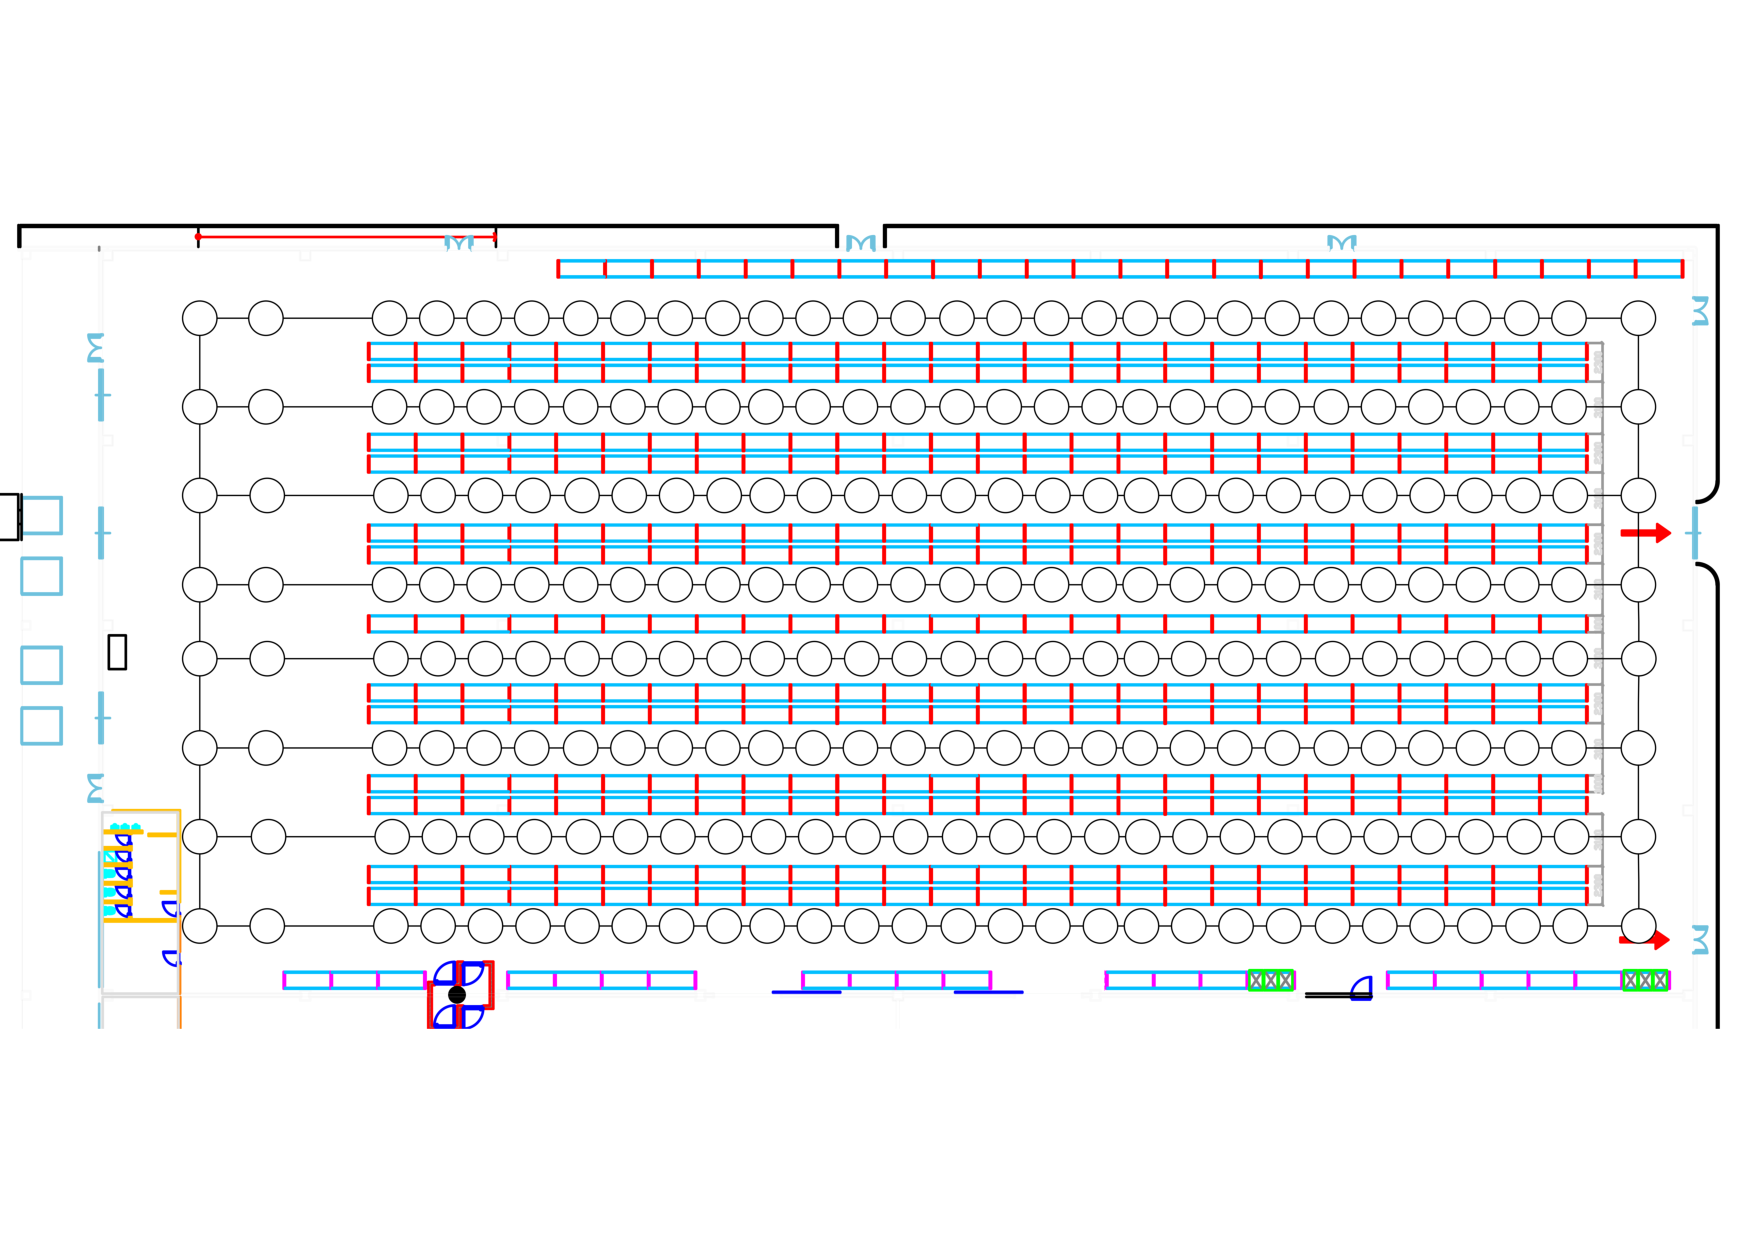
\includegraphics[width=0.8\textwidth]{mag1}
  %\includegraphics[width=0.8\textwidth]{example-image-b}
  \caption{The first portion of the warehouse to be analyzed.}
  \label{fig:mag1}
\end{figure}
\begin{figure}[tb]
  \centering
  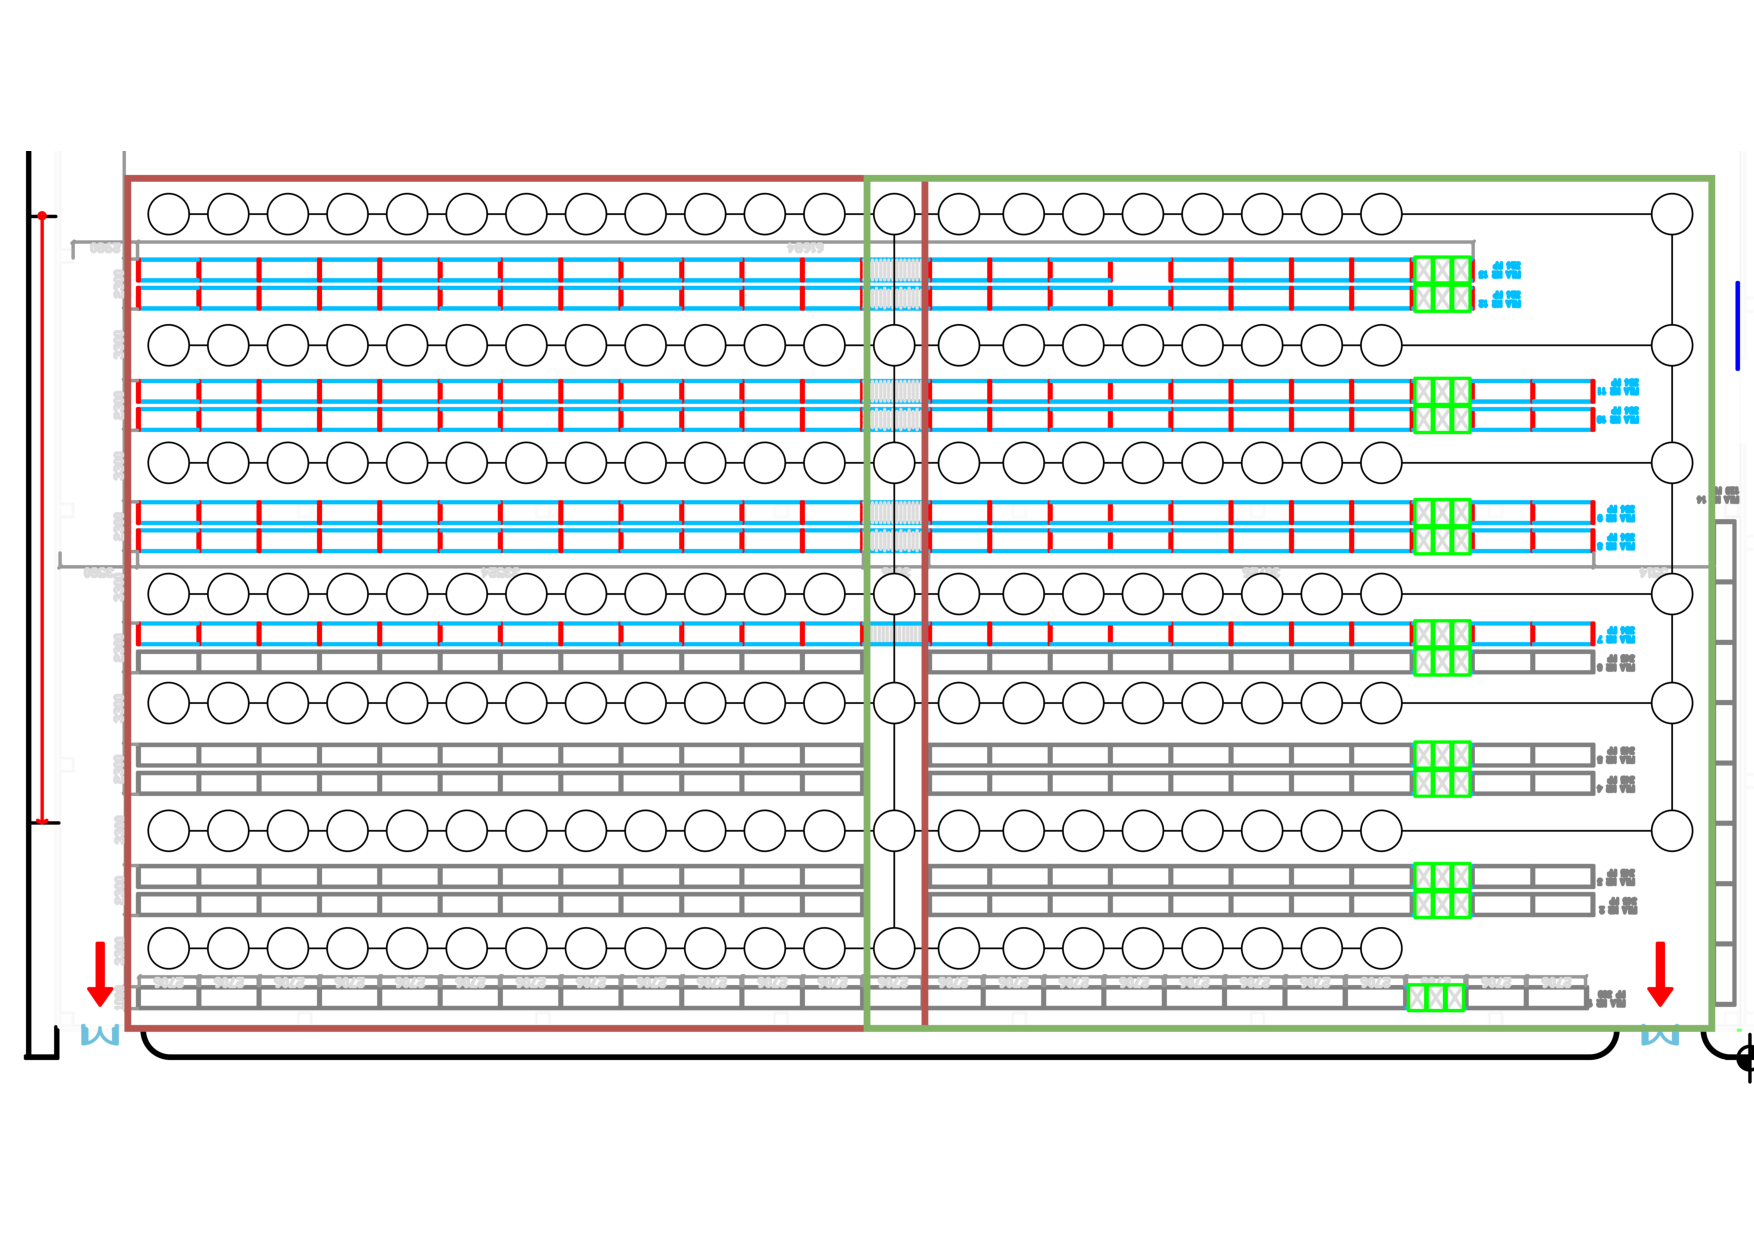
\includegraphics[width=0.8\textwidth]{mag2}
  %\includegraphics[width=0.8\textwidth]{example-image-c}
  \caption{The second portion of the warehouse to be analyzed.}
  \label{fig:mag2}
\end{figure}
Differently from the random generated tests, the warehouse tests use an already
built graph, so there is no randomness in how the graph is constructed. The 
tests were then created by changing the number of agents and the number of
goals in the test. Obviously, as for the random tests, also in these cases, 
the initial, final and goal positions were randomly extracted from the set of
nodes with the limitation that a goal position cannot be a final position.
\newline
In addition to \texttt{MAG1}, \texttt{MAG2} and the whole warehouse (namely
\texttt{MAG12}), we obtained 6 more graphs from the map to check how the
dimension of the graph impacts on the performances:
\begin{itemize}
  \item \milc{MAG2_1}: the red rectangle in Figure~\ref{fig:mag2};
  \item \milc{MAG2_2}: the green rectangle in Figure~\ref{fig:mag2};
  \item \milc{MAG2_1_1}: the blue part of \milc{MAG2_1}, i.e., the first 4 rows
    of nodes of the red rectangle, in Figure~\ref{fig:mag2};
  \item \milc{MAG2_1_2}: the grey part of \milc{MAG2_1}, i.e., the first 4 rows
    of nodes of the red rectangle, in Figure~\ref{fig:mag2};
  \item \milc{MAG2_2_1}: the blue part of \milc{MAG2_2}, i.e., the first 4 rows
    of nodes of the green rectangle, in Figure~\ref{fig:mag2};
  \item \milc{MAG2_2_2}: the grey part of \milc{MAG2_2}, i.e., the first 4 rows
    of nodes of the green rectangle, in Figure~\ref{fig:mag2};
\end{itemize}





